\listfiles
\documentclass[a4paper,pt12]{article}
\usepackage[utf8x]{inputenc}

\usepackage[english]{babel}
\usepackage[pdftex]{graphicx}
\usepackage{amsmath}
\usepackage{pdfpages}
\usepackage{fancyhdr}
\usepackage{anysize}
\usepackage{subfig}
\usepackage{graphicx}
\marginsize{2,5 cm}{2,5 cm}{2,5 cm}{2,5 cm}
\usepackage[numbers]{natbib}
\bibpunct{(}{)}{;}{a}{,}{,}
\usepackage[colorlinks=true,allcolors=black]{hyperref}
\usepackage{booktabs}
\usepackage{numprint}
\usepackage[parfill]{parskip} % linje i stedet for indent i ny paragraf
\usepackage{setspace}
\onehalfspacing

% sånn at jeg får code highlighting (måtte legge til javascript manuelt)
\usepackage{listings}
\usepackage{color}
\definecolor{lightgray}{rgb}{.9,.9,.9}
\definecolor{darkgray}{rgb}{.4,.4,.4}
\definecolor{purple}{rgb}{0.65, 0.12, 0.82}
\lstdefinelanguage{JavaScript}{
  keywords={typeof, new, true, false, catch, function, return, null, catch, switch, var, if, in, while, do, else, case, break},
  keywordstyle=\color{blue}\bfseries,
  ndkeywords={class, export, boolean, throw, implements, import, this},
  ndkeywordstyle=\color{darkgray}\bfseries,
  identifierstyle=\color{black},
  sensitive=false,
  comment=[l]{//},
  morecomment=[s]{/*}{*/},
  commentstyle=\color{purple}\ttfamily,
  stringstyle=\color{red}\ttfamily,
  morestring=[b]',
  morestring=[b]"
}

%\usepackage{harvard}
\newcommand{\HRule}{\rule{\linewidth}{0.5mm}}
\begin{document}

\begin{titlepage}

\begin{center}


% Upper part of the page
\href{http://feedjam.thunemedia.no}{
\includegraphics[width=0.5\textwidth]{figures/feedjam.png}}\\[1cm]

\textsc{\LARGE University of Bergen}\\[1.5cm]

\textsc{\Large INFO323 Semester Project}\\[0.5cm]


% Title
\HRule \\[0.4cm]
{ \huge \bfseries FeedJam: a Twitter PageRank experiment}\\[0.4cm]

\HRule \\[1.5cm]

% Author and supervisor
\begin{minipage}{1\textwidth}
\begin{center} \large
\emph{Authors:}\\
Torstein \textsc{Thune}, Lisa \textsc{Halvorsen}, Snorre \textsc{Davøen}
\end{center}
\end{minipage}


\vfill

% Bottom of the page
{\large \today}

\end{center}

\end{titlepage}

\begin{abstract}
FeedJam is an experiment where we try to combine the PageRank algorithm and a novel presentation format in order to ease digestion of large conversations on Twitter. Through employing the Kanban development methodology and the Spring framework we created a fully working prototype.

The aim of the project is to implement a version of the PageRank rating algorithm to Twitter tweets, and present the result in a novel way. The software development method we will be using to develop the project is Kanban. We will develop a high fidelity working prototype using the Spring framework. It will retrieve tweets based on the user’s search query, rank the results using the PageRank algorithm and display the results in a website.     

\end{abstract}
\newpage

\tableofcontents
\newpage

\section{Introduction}
\label{sec:introduction}
Twitter is a website where people can share short text messages about everything from simple personal doings to live reports from emerging world news stories (Twitter, 2012). Although much important information is often passed through Twitter, both as original tweets and retweets, it is often hard to follow the course of the discussion or information sharing when subscribing to certain topics due to the sheer number of tweets. Now, imagine if you could go to a specialised search engine, type in a topic or a user and then get an overview of the relevant Tweets rated by importance.

Our project “FeedJam” utilises the power of the Java MVC; Model, View and Controller; Spring framework, jQuery, HTML 5, CSS3, JavaScript AJAX techniques and the Twitter REST api and our own ranking algorithm in order to search, retrieve, rank and display tweets and their respective users. In order to alleviate the effect of limitations in the Twitter api we use caching techniques, namely caching results in a MySQL database. The application can be deployed to both Jetty and Apache Tomcat web servers running on any Unix-based or Windows NT-based systems.

In this report we will present the initial goals of the project in greater detail (section~\ref{sec:goals}), with a focus on the page rank algorithm and a novel presentation format. The report will also go into some detail about the underlying theory of ranking in web retrieval and presentation of search results (section~\ref{sec:background}). The application will also be fully detailed in the report, providing information about architecture, implementation of an standard page rank algorithm in a new setting, and a novel layout for presenting search results (section~\ref{sec:application}). A small team and complex functionality require a agile development methodology and the right software technology. Section~\ref{sec:development} will give an overview of these subjects. While developing FeedJam we ran into several problems. One of them was the practical implementation of the user rank algorithm. Because these problems were a major difficulty in the development process we dedicated a own section to them (section~\ref{sec:problems}). Last but not least, our report will summarise our level of reached goals (section~\ref{sec:levelOfReachedGoals}) and go into possible and/or interesting feature research areas that could benefit or be related to our system (section~\ref{sec:futureResearch}).


\section{Goals}
\label{sec:goals}
When we landed on the FeedJam project, i.e. to make a new website for Twitter searches, we defined two primary goals and some subsidiary goals. Our first primary goals involved investigating wether the Google PageRank algorithm could be used on Twitter users and implementing an algorithm that could do this. Our second primary goal was to make a novel layout that would make it easier to gain an oversight of and read large collections of tweets. In addition to these primary goals we defined, over time, several subsidiary goals based on personal motivations and requirements that arose during the project life cycle. These goals were:

\begin{description}
  \item[Twitter API:] To connect to and use the Twitter API to acquire search results as well as information on users and trending topics.
  \item[Spring:] To implement a web application with the Spring framework.
  \item[AJAX in Spring:] Explore the possibility of using AJAX techniques with the Spring framework.
  \item[Caching:] Implement caching of applicable items received from the Twitter API.
  \item[User evaluation:] To evaluate the resulting web application.
\end{description}

\subsection{Motivation} %lisa
%personlig: sociale media er i winden. det vil være inteeressant å  gjøre noe med ir for sosiale medier.
Our personal motivation for making FeedJam was that we got the chance to acquire new programming skills. We feel it is easier and more inspiring to learn about techniques in the information retrieval field when we can use the theories in a practical sense. Twitter was chosen as a domain because social media and micro blogging are popular research fields. We also wanted to explore their API and see if we could make something interesting and enhance the application using theories from the information retrieval field.

%faglig: lære mer om hvordan søkemotorer ranker ting, presentasjon. Lære med om verktøy som brukes. Er det et behov for å gjøre dette?
PageRank has seen great success as a ranking algorithm for general web search, popularised trough Google's own search engine. The scientific motivation behind FeedJam is to see if the page rank algorithm is feasible and applicable to a social network, and if the ranking algorithm and a new way of presenting search results will make it easier to get a quick overview of the important tweets in the feed.

\section{Background}
\label{sec:background}
%teoridel
In this section we will present some background information about the topics that the project consist of. We'll star by introducing ranking in relation to search engines. After this we will take a closer look at the algorithm that we will use in our project, the PageRank algorithm.  Following will be a short introduction to Twitter, the social media that is the domain of the project. The section will finish with a presentation of some related work and a subsection of your motivation for doing the project. The next section .....


\subsection{Ranking} 
In defining the goals for this project we chose to focus on two parts of the web information retrieval process, ranking and presentation of search results. Ranking is the hardest and most important function of a search engine \citep[p.469]{Baeza-Yates2011}. One of the key challenges in ranking, according to \citet{Baeza-Yates2011}, is to identify quality content on the web. Evidence of quality can be indicated by several signals such as domain names [...], text content, and various counts (such as the number of word occurrences), links (like PageRank), and Web page access patterns as monitored by the search engine” \citep[p.468]{Baeza-Yates2011}. 
\citet{Baeza-Yates2011} go on to describe different types of signals that can be used to improve ranking of web results. These will be briefly described here. Content signals refers to the content of the document, mainly text. The signal in the content type refers to things such as word counts, vector space model-based scores and so forth. Structural signals, according to \citet{Baeza-Yates2011}, includes signals such as the links on a page, the text in anchor elements, and in and out-links to a page.  The last signal type describes is the web usage signals. User clicks is one often used signal where the relevance of a result is affected by the number of clicks it receives. Other signals mentioned are geographical location, language, technological context and temporal context (that is web usage over time gathered through cookies or user profiles)\citep{Baeza-Yates2011}.

Content signals will be used in FeedJam's TweetRank. We will explain in more detail about how we use hashtags, mentions and retweets to create a score in section \ref{} \nameref{}

Link-based ranking is based on using structural signals (i.e. counting the number of outgoing and incoming links on a page) to rank a page or document. One ranking algorithm based on this  principle is the Google PageRank algorithm \citep{Page1999}. We will use this to create a UserRank for Twitter users. 

\subsubsection{Page Rank}
%something about that pagerank comes from the idea of citations counting in journals. If a journal is cited in many articles it is most likely an important article. PageRank takes this idea one step forther. 
The goal of the PageRank ranking algorithm is stated as follows: “This ranking called PageRank helps search engines and users quickly make sense of the vast heterogeneity of the World Wide Web” \citep[p. 1]{Page1999}. It derives from citation counting which is a way tell the importance of an article. An article that is cited by many other articles is most likely an important one. 

The PageRank algorithm exploits the structure of the web in the calculation of the rank. The World Wide Web can thus be viewed as a graph with directed edges between nodes. The edges are either links pointing to the page - we call them back-links. Or they are links pointing to another page - called outgoing-links or forward-links. Looking at the structure of the web and trying to create a ranking of web pages, \citet{Page1999}%Page and ... \citet{} 
took the idea of citations counting one step further. In addition to the number of web pages that point to a page, it also looks at the actual pages that link to it. 
\citet{Page1999} noted that giving high ranks just by looking at the number of back-links (incoming links) is problematic because a site might get many back-links from various web pages that are not very important. They provide a solution to this by proposing that not only the number of back-links, but also the rank of the web pages for these back-links can be used when ranking a web page. Given this solution, as shown by \citet{Page1999}, a page receives a high page rank if the sum of the sum of the page ranks of the back-links is high.

The PageRank algorithm simulates a user navigating through the web randomly. The user is currently at page a. From here she randomly clicks on one of the links on page a to get to the next page. The process is repeated. Using the pattern created by many numbers of clicks by the user, it is possible to compute the probability of which the user has visited each page. There are some restrictions to the computation. The web has pages without outgoing links and self-links where the user is not able to move on. Another hensyn we have to consider is the probability that the user moves to another page not using the links on the current page. Med disse hensyn PageRank is calcualted as follows.
Let L(p) be the number of outgoing links of page p and let p1 . . . pn be the pages that point to page a. q is the probability that the user jumps to another page and 1-q is the probability that she follows the link.  Then the PageRank of page a is given by the probability P R(a) of finding the user in that page
P R(a) = q/T + (1 − q)
Xn
i=1
P R(pi)
L(pi)

where\newline
T: total number of pages on the Web graph\newline
q: parameter set by the system (typical value is 0.15) \newline
When computing the algorithm we have to consider the problem of pages with no outgoing links. \citet{Baeza-Yates2011} propose two solutions. One is to put q = 1 for thses pages, the other is to leave them out, and compute their rank at the end based on their parents rank. 


\subsubsection{User Interface}

{\bf Interaction design principles and user-centered design}\newline
Within the field of interaction design we have several different design guidelines and principles for creating usable artefacts. \citet{Sharp2007} name visibiity, feedback, constraints, consistency and affordance as the essential design principles.

\begin{description}
  \item[Visibility] bob kåre
  \item[Feedback]  :D
  \item[Constraints] :D
  \item[Consistency] :D
  \item[Affordance] :D
\end{description}

In addition to exploring ranking algorithms we are going to develop a novel interface to display tweets and their rankings. In the book Interaction Design: Beyond Human-Computer Interaction Sharp et al (2007) present several factors who are paramount to good interaction design. In order to design good interaction one should take into account the usability principles as presented in the book. These are visibility (whether the functions/input mechanisms are visible or hidden), feedback (the interface should show that the system has received and used the input given), constraints (avoiding facilitating invalid user input for given contexts), consistency (similar operations use the same kinds of elements) and affordance (whether users can use familiarisation from experience in order to naturally understand what the interface element does). In addition to this the book also provides a set of metrics which can be utilised to measure the usability of an artefact.\newline

{\bf \noindent Classic search engine result pages}\newline
\citet[p.480]{Baeza-Yates2011} argues that existing search engines are heavily influenced by what they call a extreme simplicity rule. Basically this rule states that search engine user experience must be simplistic enough in nature that users understand it without any previous knowledge, or else they will simply switch to another search engine. This has lead to a very prominent interface paradigm where all the most prominent search engines use the classic search engine result page (SERP) \citep{Baeza-Yates2011}. 
As search engines have started to search several different content types the need to display several different media types in one unified result page have also emerged. This has resulted in two innovations: the “onebox” \citep{Baeza-Yates2011}, which displays specific information from one knowledge domain (e.g weather reports) and universal search results where one combines several different searches into one search result page.


\subsection{Twitter}

\label{Twitter}
%litt om hvordan twitter kan være vanskelig å få oversikt over en strøm. finn statistikk om megden tweets i døgnet.

%vi kan tilby noe mer enn twitter search enginen gir. Vi tilbyr en mer oversiktlig tjeneste. 
%se om det finnes noe som sier noe om hvordna brukere bruekr twitter. 
When deciding what information retrieval (IR) techniques we could apply to Twitter we found that when searching for Tweets it not easy to see what tweets are important and which are not. If you search for at certain topic on Twitter you get at feed of all tweets that match the search query. It can be some users personal diary, a conversation between users, information sharing or spam. Following we wanted to use IR techniques to make it easier to see what Tweets are important. 

Twitter is a microblogging service available for more than 20 languages \citep{Twitter2012}. User post messages, called tweets, about what they find interesting which are read by other users. As Twitter has become popular it has received a broad user group. The difference between Twitter and other social networks is the way  that it defines the relationships in the network. On Twitters a user is following other user and is being followed by other users. The difference is that the relationship doesn't have to be reciprocal. Being a follower means you receive all the tweets of the users you follow. \citep{Kwak2010} finds that 77.9\% of the followers relationships on Twitter are non reciprocal. This is one of the features we will take advantage of in order to rank tweets. 

\citep{boka kap11} Noe om distribusjonen av sider og linker på web i kap 11. .. noe om zipf lov. Pareto distribution similar to the power law. Many small documents Det samme gjelder for Twitter?

%Dette var noe jeg fant i en artikkel. OG det er ikke så vanskelig å implementer noe som sier om en bruker er venn, deler eller søker. Kanskje vi skal gjøre det?
Users use Twitter in different ways. \citet{Akshay2007} finds three man user categories: Information source, Friend and Information Seeker. Information sources are user that updates their status with regular intervals and has many followers. The number of followers is due to the value of the information they give through the Tweets. The Information Seeker is a user who rarely post Tweets, but follows other users on a regular basis. A Friend is a users with many reciprocal relationships. We may use these user categories in the UserRank. 

Twitter also has other features that can be used in ranking. Important words in the text of a tweet can be marked with a hash tags ("\#" ). Tweets can be retweeted which is a mechanism that empowers the spreading of the tweet. \citep{Kwak2010} finds that a retweeted tweet reaches an average of 1000 users no matter what the number of followers the author of the original tweet has. 

We used the Twitter REST API to retrieve tweets and user information. More on how we used it can be found in section \ref{} \nameref{} 

%Lisa: flytta technologies delen til development delen. Føler det hører mer hjemme der.



\subsection{Related Work}
{\bf trst.me} \newline
trst.me \citet{Infochimps2012b} is tool for measuring a Twitter user's reputation. The measure is two dimensional and consists of the Trstrank and the Trstquitient. The Trstrank is a implementation of Google's page rank \citep{Infochimps2012a}, the same rank the FeedJam uses for the userRank. The Trstrank gives a score between 0 and 10 which gives many users the same rank. To differentiate between the users trst.me uses the Trstquotient. It is "an integer between 0 and 100 that quantifies the relationship between a user's Trstrank and their followers count"\citep{Infochimps2012}. The quotient is used to separate spammers from quality users. 

trst.me compared to FeedJam is just a service for finding a Twitter user's trustworthiness. It allows users to enter the screen name of a Twitter user and returns their rank along with other related metrics.  

\subsection{Motivation} %lisa
%personlig: sociale media er i winden. det vil være inteeressant å  gjøre noe med ir for sosiale medier.
The personal motivation for doing this assignment is that we got the chance to acquire new programming skills. We feel it is easier and more inspiring to learn about techniques in information retrieval field when we can use the theories in a practical sense. Twitter was chosen as a domain because social media and microbloging is a poplar research field. And we wanted to explore their API and see if we could make some interesting and enhance the application using theories from the information retrieval field. 

%faglig: lære mer om hvordan søkemotorer ranker ting, presentasjon. Lære med om verktøy som brukes. Er det et behov for å gjøre dette?
Social media are growing in popularity...



\section{The application}
\label{sec:application}
%Short description of the posible actions in feedjam
In this section we will describe the finished FeedJam application.
%Sections
\subsection{Structure}

\subsubsection{MVC} %torstein view delen, lisa model og contoller
The application is built on Spring's Web MVC framework. MVC separates the business logic from the user interface through the controller that handles the communication between the two. The Spring MCV is request driven and designed around Springs Front Controller the DispatcherServlet that dispatches requests to controllers and offers other functionalities that facilitates development of web apps. The request goes through following steps:

\begin{itemize}
\item Client sends a request to the web container in the form of a http request
\item The request is handled by the DispatcherServlet which finds the appropriate Handler Mapping
\item The Handler Mapping helps the DispatcherServlet send the request to the right Controller. 
\item The controller processes the request and returns a view in the for of a ModelAndView instance that's sent to the DispatcherServlet. 
\item The DispatcherServlet resolves the view by consulting the View Resolver
\item And the view is then returned to the client. 
\end{itemize}

--------- TODO ---------- 


\subsubsection{The Model} %what it does. what is contains 
The model is the part of the application that contains the domain objects or the core data structures. In FeedJam the main interfaces are TwitterUserInfo323, TweetInfo323 and Trend. Trend represents the trending topics presented on the front page. While TwitterUserInfo323 represents the user including the information such as name, screen name, number of followers and following, tweets count etc. It also contain a field for fitnessScore which represents the user's UserRank. TweetInfor323 represents the tweets and info related to them. Some of the fields are text, retweetCount, tags, mentions and tweetRank. The TweetObject also contains reference to the Twitter user that wrote the tweet (the field userInfo). Trends, TweetSearchResult and FollowersFollowingResultPage are interfaces used to create the object that are sent to the view. 

A factory pattern is used to create the objects needed in for the persistence layer. 
More info about the connection can be found in section \ref{sec:feedJamDatabase} \nameref{secc::feedJamDatabase}.


--------- TODO ---------- 

\subsubsection{The View}
The view is the component of MVC-applications which receives input from the user and displays output from the controllers and model. While the model and the controllers contain logic in order to do database interactions and data manipulation the view in general only contains logic in the form of simple if-statements and loops in order to display the content assigned by the controller. The view is also the component which, in web applications, contains the HTML markup, CSS-styling and Javascript needed to provide users with the intended graphical design and user experience.

Within the context of Spring, views are written in a language called JSP. JSP, Java Server Pages, is an alternative form of Java intended to be used to print variables within HTML. Unlike many other languages used for web programming like PHP, JSP pages are pre-compiled. While it is possible to write entire applications in JSP it is generally not considered good practice to write any logic outside logic specifically needed in order to display content from within the objects assigned to the view by the controller.

\subsubsection{The Controller}
%FeedJam has two controllers, HomeController and AjajController, one for each view in the application.
The controller takes the user input from the view and sends it to the business logic that handles it and sends response back to the controller \cite{}. The controller receives request from the view in an JSON format. The JSON string is parsed by a JsonParser (utils-package) and the model produces a response. The controller prepares a Map (footnote java.util.Map) containing the view(s) and the response objects. A Spring InternalResoucesViewResolver generates the view with information  from the Map.

--------- TODO ---------- 

%hva MVC er
%hvor ting er
\subsubsection{Interaction between view and controller} %snorre
\label{viewControllerInteraction}
When the user searches for a term on FeedJam a complex series of interactions happen between the view/the users browser and the FeedJam server. These interactions are illustrated in Figure~\ref{fig:AjaxInteractions}. When the user enters a search term into the FeedJam searchbox and clicks the search button the entered term is snapped up by Javascript. This search term is then, along with some other variables such as the number of tweets to fetch, formed into a GET request to the Twitter search API. The returned JSON is then sent to the AJAJ controller, which parses the JSON and generates a list of users whom are not in the database/or have not been updated for several weeks. This list of users is then returned to the client.

\begin{figure}[ht]
    \begin{minipage}[b]{1\linewidth}
        \centering
        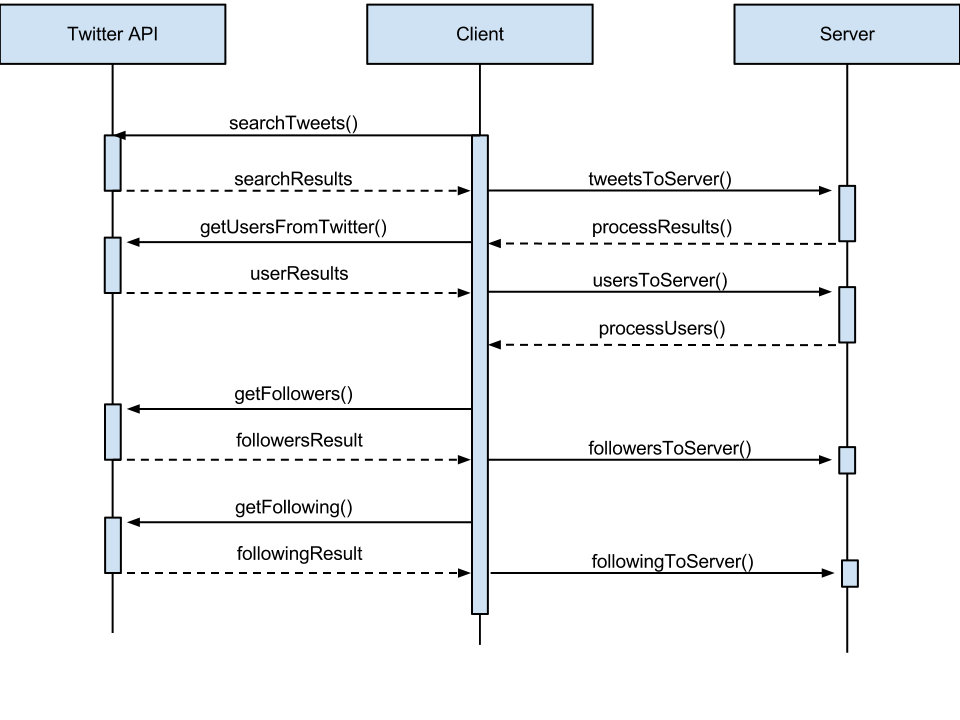
\includegraphics[width=1\textwidth]{figures/sequencediagram}
        \caption{Sequence diagram for ajax interactions between browser, server and Twitter.}
        \label{fig:AjaxInteractions}
    \end{minipage}
\end{figure}

\begin{figure}[h!]
\begin{lstlisting}[language=javascript]
// sends following to controller (ajaj/processFollowing)
function followingToServer(userId, followingData) {
  $.post("ajaj/processFollowing", 
  { 
    userId: userId.toString(), // server wants userId as a string
    following: JSON.stringify(followingData) // and JSON as a string
  },
  function(data) {
    console.log("SERVER RESPONSE: added following for " + userId);
  });
}
\end{lstlisting}
\caption{Example jQuery code for sending following for a user as JSON to the controller}
\label{ajaxRequest}
\end{figure}

The client then requests user information about all these users from Twitter. The returned JSON-formatted user data is then forwarded to the controller along with the previously returned JSON-formatted tweets. The reason why we return the tweets a second time is due to the fact that we do not formulate a session for each search, thus rendering the controller unable to couple the two HTTP POST requests with eachother. The controller then processes the tweets and the returned users and finally returns a finished view as HTML to the client. This finished HTML is then dynamically appended to the tweet grid using Javascript.

After the generated view has been inserted the client starts requesting followers and following for each of the users who were looked up. This is done this lately in the process in order to ensure that the view is returned and displayed to the FeedJam user as soon as possible, thus making the system appear faster. Since we are using AJAX this can be done behind the scenes without the user noticing. Each response from the Twitter API is then asynchronously sent to the controller, which in turn processes the JSON and inserts the values into our database.

\subsubsection{Interaction between controller and model} %lisa
%information flow, hvordan ting skjer
FeedJam has three controllers. The HomeController handles the trend requests for the front page. It finds the time of the request and uses the MySQLTrendingFactory class to search the database for trends. If the trends exists in the database they are returned to the view. If trends for the current hour does not exist in the DB, a request is sent to the  Twitter API. The response is stored in the database and sent to the view. More on the database in section \ref{feedJamDatabase} \nameref{feedJamDatabase}.

The AjajController handles all search requests. When the client has retrieved search results from Twitter, the JSON response is posted to AjajController. Using the MySQLUserFactory, it queries the database to check if user information of the tweet owners is cached. If some users are not recorded in the database, a response is sent to the view. It contains a JSON array of users the client needs to retrieve information about. 

The AjajConntroller then receives a POST containing the the information on the remaining users information. New users and the Tweets are inserted to the database and a TweetSearchResult object is created. The result contains the requested Tweets with associated user information. The result is then sent as a response to the view. When the client has received the response from the server it requests the users' followers and following. The list containing these users is sent to AjajController which uses MySQLUserFactory to insert them into the database. The application logic for this operation is listed in Figure \ref{javaProcessFollowing}.

\begin{figure}[h!]
\begin{lstlisting}[language=java]
@RequestMapping(value = "/processFollowing", method = RequestMethod.POST)
public ResponseEntity<String> processFollowing(
  @RequestParam String userId,
  String following) 
  {
    long userIdLong = Long.parseLong(userId);
    
    // Parse the json string and store following in result page object
    FollowersFollowingResultPage followingResultPage = 
      JsonUserParser.jsonToFollowersFollowing(userIdLong, following);
    
    // Insert following objects into database
    int updated = 
    mySqlUserFactory.insertBatchFollowing(followingResultPage);

    // Return a HTTP OK status to the client				
    return new ResponseEntity<String>(HttpStatus.OK);
}
\end{lstlisting}
\caption{Example Java code for receiving and inserting following into the database.}
\label{javaProcessFollowing}
\end{figure}

The SearchController is now used as a backup. It originally handled server side requests to Twitter. As explained in section \label{twitterProblem} we had a large amount of problems connected with the limited amount of requests per ip-adress per hour. Since the SearchController performed API requests server-side this meant that FeedJam could serve a maximum of 150 searches per hour in total. While all API requests are handled client-side in the final FeedJam version we keep the SearchController as a backup in the cases where the users have disabled Javascript in their browser in order to provide a similar, though limited, experience for those users.

%brukt desingn patterns 

{\bf packages}
\begin{itemize}
  \item uib.info323.twitterAWSM contains the controllers
  \item uib.info323.twitterAWSM.exceptions contains exceptions
  \item uib.info323.twitterAWSM.io contains interfaces for interacting with persistence layer (postfixed -DAO), interfaces for searching the Twitter API (postfixed -SearchFactory) and interfaces for crating model object (postfixed -Factory).
  \item uib.info323.twitterAWSM.io.impl contains MySql implementations, Json implementations and model implementations. 
  \item uib.info323.twitterAWSM.io.rowmapper contains rowmappers used in accessing persistence layer
  \item uib.info323.twitterAWSM.model.impl contains model implementations
  \item uib.info323.twitterAWSM.model.interfaces contains model interfaces
  \item uib.info323.twitterAWSM.model.impl contains model implementations
  \item uib.info323.twitterAWSM.pagerank contains PageRank/UserRank implementation
  \item uib.info323.twitterAWSM.model.utils contains parsers etc.
\end{itemize}

\subsection{Layout} %torstein
A large part of our project was to develop a novel way of displaying tweets. This section will explain how we developed the layout concept in addition to explaining how we implemented it using modern standards and techniques.

\subsubsection{Defining the concept}
Since FeedJam is an effort to ease the consumption of tweets and Twitter conversations through the use of the PageRank algorithm, to rank users, and a simple tweet ranking we needed a good way of displaying the results of said rankings graphically. Normally search engines are able to sort the output of searches after relevance due to their non-restricted access to their own database. However, in the case of Twitter, we only have access to a limited number of tweets through their public API. In addition to this we believe that the sheer amount of new tweets every minute would be a too large to effectively process for our equipment even if we were able to fully access the Twitter database. Therefore a normal sorted listing of search results were effectively rendered impossible. Another aspect to take into consideration is the conversational nature of many tweets. It was decided that the FeedJam layout would somehow follow the conversation without sorting tweets but simultaniously helping users skim through large conversations quickly and help users see important tweets.

Normally when browsing through lists of unsorted rated content we are explicitly shown the content's rating. This is true for instance in the case of movie or music listings where a grade is displayed, often in the form of a dice or a number. While we did want to display our rating we also wanted to provide the user with more powerful visual cues to the generated importance measure of tweets in order to follow our layout goal of easing skimming of large conversations. Hence we decided on the use of purely visual cues in the form of colours or transparency in order to differentiate between rankings.

\subsubsection{Early efforts}
Early concepts placed tweets in a list format. The thinking behind using a simple list format is that Twitter in its current iteration use a similar design to display tweets. This did however prove to be an inefficient use of the available space in the browser, and was quickly scrapped in favour of a grid-based layout.

\begin{figure}[ht]
    \begin{minipage}[b]{0.5\linewidth}
        \centering
        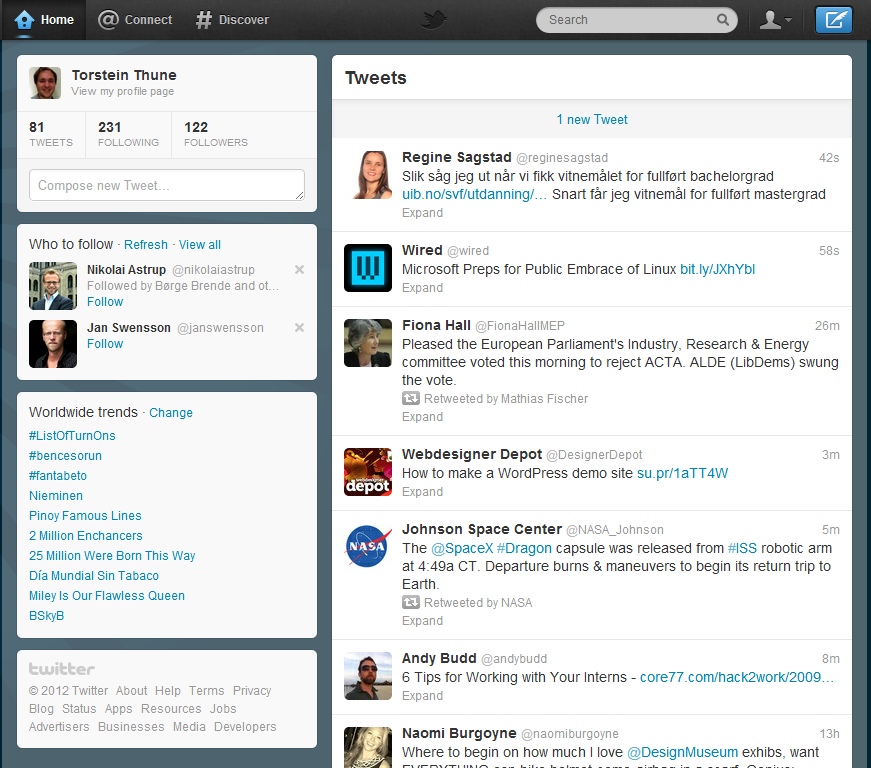
\includegraphics[width=\textwidth]{figures/twitter_list}
        \caption{Twitter in its current iteration.}
        \label{fig:Twitter}
    \end{minipage}
    \hspace{0.5cm}
    \begin{minipage}[b]{0.5\linewidth}
        \centering
        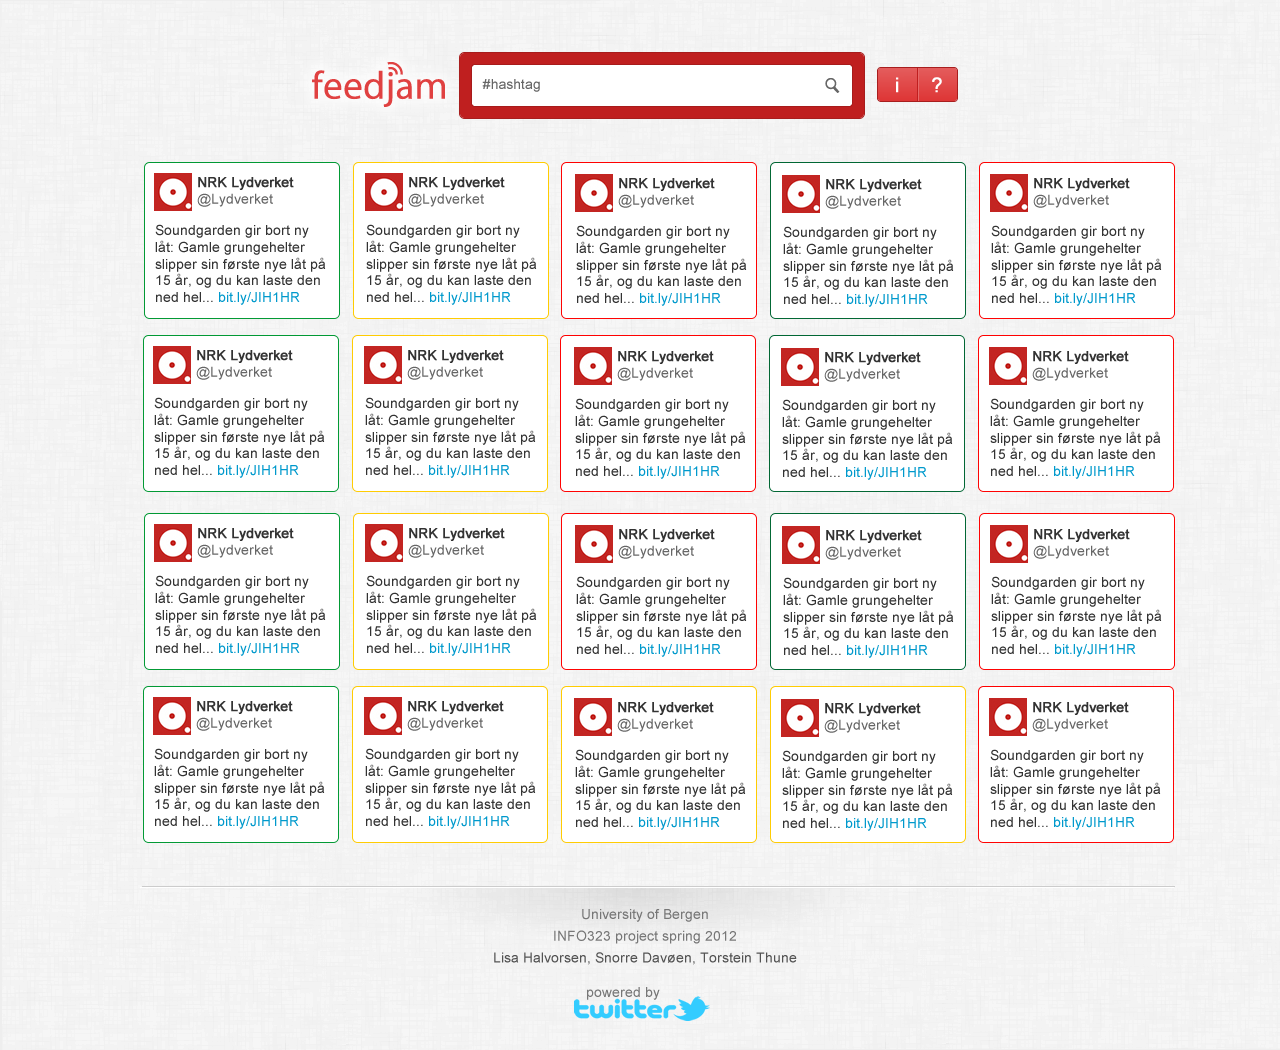
\includegraphics[width=\textwidth]{figures/layout_colour_borders}
        \caption{Early FeedJam concept}
        \label{fig:FeedJamColours}
    \end{minipage}
\end{figure}

We did also experiment with using colours to display the importance of tweets. Early thoughts used a traffic light metaphor where green signalised a good ranking, yellow a neutral ranking and red a bad ranking. The colours were used as border-colours, as seen in figure  \ref{fig:FeedJamColours}. This did however prove to be a too insignificant visual cue, leading to it taking too much cognition to perceive the actual ranking of tweets. While it could be argued that one with some training would be able to lessen the cognitive burden of this design, we decided that we wanted an even easier ranking layout concept. Another problem  with the traffic light metaphor was that we were only able to create three ranking brackets, which took away from the nuances of our ranking algorithm.

\begin{figure}[ht]
    \begin{minipage}[b]{1\linewidth}
        \centering
        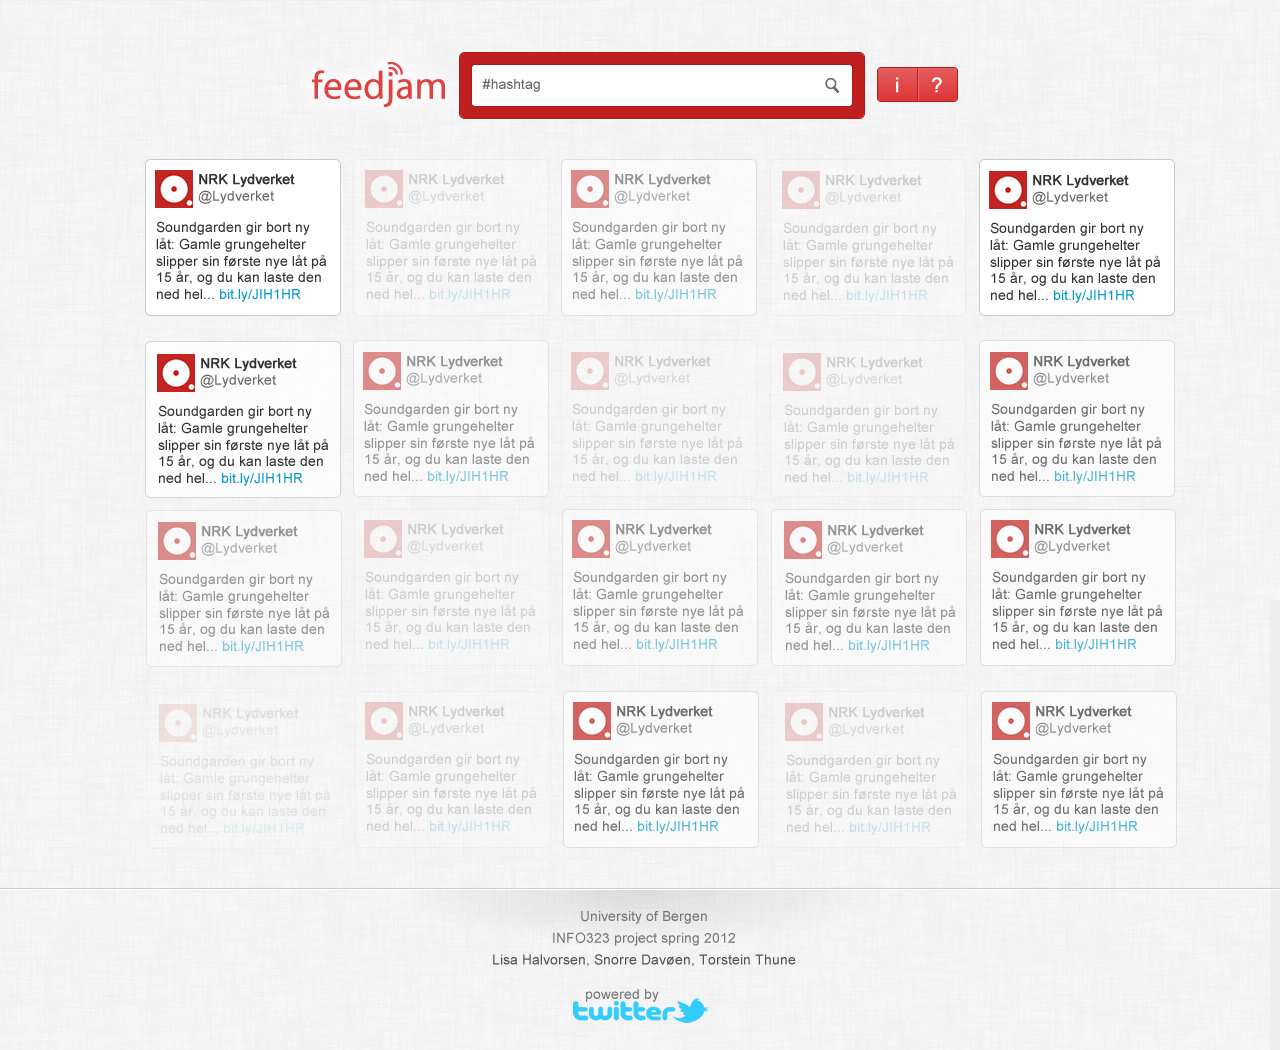
\includegraphics[width=0.5\textwidth]{figures/layout_transparency}
        \caption{FeedJam concept using transparency}
        \label{fig:FeedJamTransparency}
    \end{minipage}
\end{figure}

Since our ranking algorithms has an output in the form of a float number (a number betweet 0.0 and 1.0) we decided that opacity, whose CSS operator can take in values in a float format, would be better suited. Using opacity we were also able to display the nuances of our ranking algorithm. We also found that this concept was less taxing cognitively, and that we were able to estimate the tweets' rankings without much cognitive thought. The best tweets, rendered completely visible, would also stand out compared with the other tweets to a much larger degree than when using the traffic light metaphor.

\subsubsection{The final layout}
When visiting the FeedJam web application the users are presented with a clean layout consisting of a logo, a search box, a list of trending tweets and a footer containing some information about the project and its creators. The colour scheme is very simplistic, relying on red and different shades of gray, resulting in a minimalistic design.

\begin{figure}[ht]
    \begin{minipage}[b]{0.5\linewidth}
        \centering
        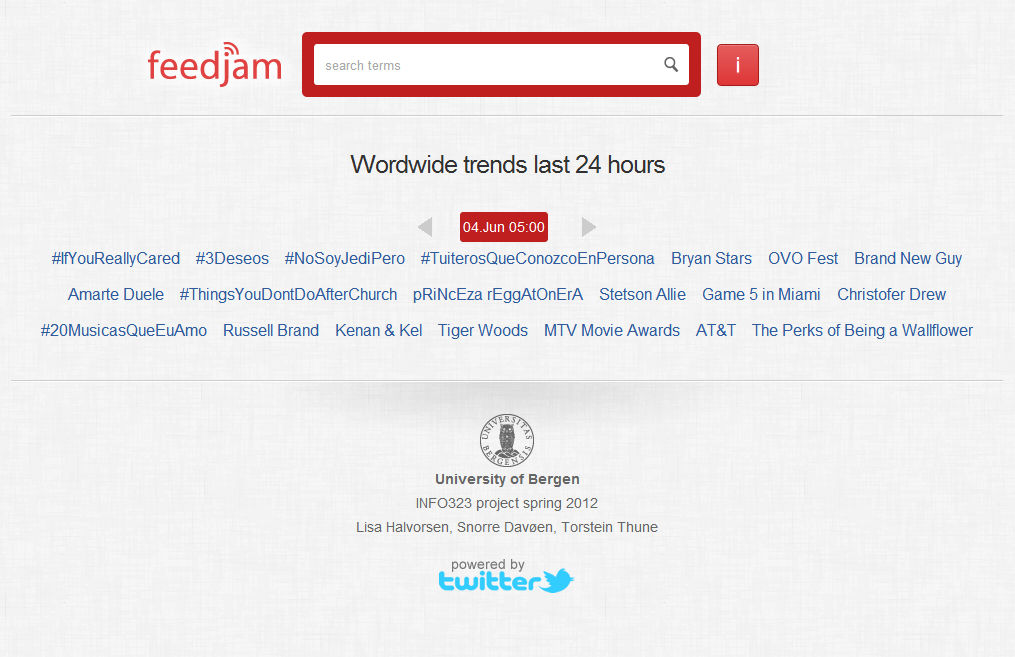
\includegraphics[width=\textwidth]{figures/feedjam_final_frontpage}
        \caption{FeedJam frontpage on laptop/desktop computers}
        \label{fig:FeedJamFrontpage}
    \end{minipage}
    \hspace{0.5cm}
    \begin{minipage}[b]{0.5\linewidth}
        \centering
        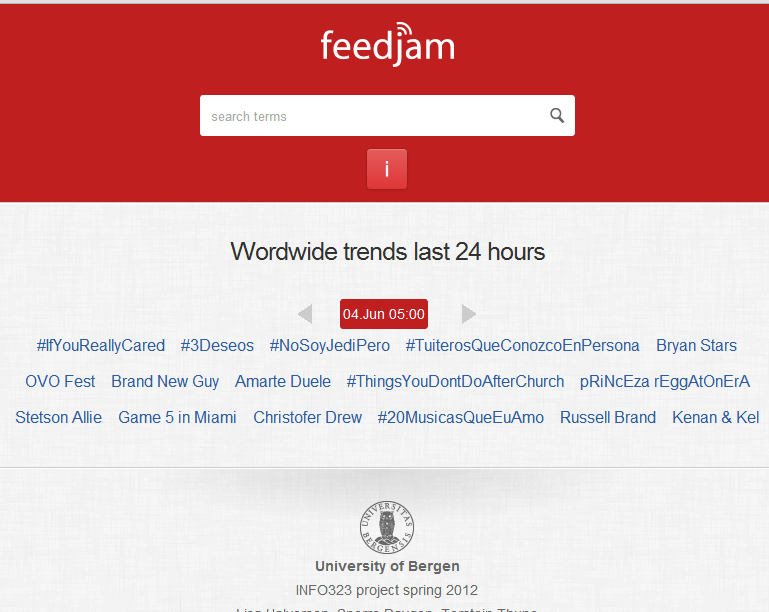
\includegraphics[width=\textwidth]{figures/feedjam_responsive_frontpage}
        \caption{FeedJam frontpage on tablets}
        \label{fig:FeedJamFrontpageTablet}
    \end{minipage}
\end{figure}

The search form consists of a standard, though large, search input field and a search button, thus providing both good visibility, since the form is very prominent, and affordance, since users are used to the concept of a search box and thus knows how to use it.

When entering a search term and clicking the search button (or when clicking a trending topic) the front page fades out, and a loading bar appears displaying information about what is being done. While the site exhibits unusual form behaviour, e.g not causing a page reload when clicking submit, this loading bar; with its connected loading messages, shows the user that something has happened and that something is still happening, thus fulfilling the feedback design principle.

\begin{figure}[ht]
    \begin{minipage}[b]{1\linewidth}
        \centering
        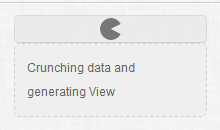
\includegraphics[width=0.5\textwidth]{figures/feedjam_loading}
        \caption{The loading bar}
        \label{fig:FeedJamLoading}
    \end{minipage}
\end{figure}


The search result page consists of a strict grid with 4 columns (or less depending on screen resolution) where each tweet is set at a specific width. Each tweet is in its own box with varying opacity depending on the relevant rankings. In order to clearly show where tweets are in the grid even at lower opacities the border is always at 100\% opacity. While some tweets are almost transparent, they will become fully visible when pointed at by the mouse pointer or clicked on tablets and smart phones. This is done in order to make all tweets readable.

When clicking a username a small modal window appears displaying information about the user, including our user rank, the number of people following the user and the number of people followed by the user, the user's description from Twitter in addition to links to his/her web page and profile. This window can be closed either by re-clicking the user name or by clicking outside the modal window.

Beneath the grid of tweets there is a "load more" button. By clicking this button the user sends an AJAX request both to twitter to get the next 20 tweets which is then sent to the server. The server in turn goes through the same steps as when using the search box, finally resulting in a generated view (a tweet-grid) which is dynamically appended to the existing grid using jQuery.

\subsubsection{Coding of the layout}
The frontend is coded using standard HTML5 for markup/structure, CSS3 for styling and Javascript coupled with jQuery for front-end scripting. In addition we use JSPs, which are in essence compiled template files, to generate the HTML displayed to the user.

The frontend is organised in several views. Roughly we can divide these views into two categories: main views and views which are included into other views. FeedJam has one main view called home.jsp. This view generates the markup which the user is presented with when he/she first visits the feedjam website. The home view also uses the views footer.jsp which contains the markup for the footer (bottom of page), htmlheader.jsp which contains javascript declarations and jQuery initialisation and header.jsp which contains the search form. Other views is the tweetList.jsp view and the trendingList.jsp view which are used to generate grids of tweets and a slider of trending topics. These are placed dynamically within the home.jsp view through the use of jQuery.

%Backend: Spring, Spring mvc, maven,  DAO, factorys, running on java servers, db more in db section,  developement
%\subsection{Backend} %Serverside?
%The application is developed in Spring MVC framework. 

%Ranking: implementation, reference
\subsection{Ranking} %lisa
\label{ranking}
The FeedJam ranking consist of two parts, the TweetRank and the UserRank. It is displayed through the opacity of each tweet. The idea is that tweets tweeted by a user with high UserRank gets a high score. Tweets by high-ranking users will have close to 100\% opacity (no transparency) unless the tweet itself contains spam signals (see more below). The FeedJam ranking will also allow for normal users who follow good tweeting practice to get a good score.

\subsubsection{TweetRank}
The TweetRank is based on the idea of using ranking signals in search engines. Even though there isn't as many content signals in a tweet as in a normal web pages we use them to make the TweetRank. "\#" symbol is used in Twitter to mark keywords or topics in a tweet \citep{Twitter}. Twitter recommends using no more than 2 hash tags in a tweet. 
Mentions are another mark-up that is used in tweets. It indicates either that a tweet is a reply to another tweet or that a tweet concerns a user \citep{Twitterb}. If a tweet is read by many, it is considered important. The Twitter API does not provide this statistic. We have decided to use the retweet count of tweets as a heuristic to get an idea of how many times a tweet might have been read.

\subsubsection{UserRank}
The UserRank uses information about a user's followers and who a user follows to rank the user. The follower relation between to users represent the back-link (or inbound link) relationship in a page rank algorithm. The following relationship between two users represents the forward link (or outbound link) relationship. If you recall the three user categories described in section~\ref{Twitter}, it is clear that a user with a high user rank (i.e. high page rank) falls under the category Information source, and should therefore be regarded as an interesting user. It is probable that a highly ranked user have many followers, the followers themselves having a high user rank, because she makes interesting tweets.

{\bf UserRank implementation}\newline
The UserRank implementation used in FeedJam is based on \citet{Goodrarzi2009}'s implementation of page ranking in Java. The first step when finding a user \emph{a}'s UserRank is to find all the followers of the user, then find their followers, etc. This is repeated until all related users are found and stored in a list (params). A matrix is then generated from the users in the params-list. Then a matrix containing a multifactor-constant is created. The multifactor is calculated based on the relations between the users, how many are following them and the damping factor (see source code UserRank.getMultiFactor). After this a matrix of 1- DAMPING\_FACTOR is made. These two matrixes makes out the linear equation that is the user's UserRank. The solving of the equation is left to a third party API \citep{Jama}. Lastly the rank of the user is picked out of the matrix.

%Litt mer om hvordan pagerank kan brukes på Twitterusers. Lage en graph/tegning. Vise at det i teorien skal oversettes - argumentere. Sosiale nettver er ganske like weben. 
%Optimalisation 
Our initial implementation of the ranking algorithm was extremely slow and ranking every user was simply not feasible due to the time requirement of the algorithm. To optimize the algorithm we performed a  simple time complexity analysis in order to identify critical operations in the ranking algorithm which could be optimised. To explain how we optimised the algorithm it is necessary to show some of the source code used in the ranking algorithm. Figure~\ref{fig:generateMatrix} shows the code that generates the matrix used in the algorithm. The generateMatrix method gets the multi factor for each cell in the matrix. The getMultiFactor method is run \(n^2\) times where n is the number of users in the parameter list.

\begin{figure}[h!]
\begin{lstlisting}[language=java]
private double[][] generateMatrix(){ 
  double[][] arr = new double[params.size()][params.size()]; 
    for(int i = 0; i < params.size(); i++){ 
      for(int j = 0; j < params.size(); j++){ 
        arr[i][j] = getMultFactor((String) params.get(i), (String) params.get(j));
      }
    } 
  return arr;
}
\end{lstlisting}
\caption{Java code for generating the linear equation parameter matrix \protect \cite{Goodrarzi2009}.}
\label{fig:generateMatrix}
\end{figure}

If one takes a close look at the original getMultiFactor method (Figure~\ref{fig:getmultifactor}) one can see that two database operations, getInbound and getOutBound, are performed for each matrix cell. This amounts to a time complexity of O(\( n^2\)) for these two database operations. If one presupposes that each database operation takes about 50 milliseconds to complete, then the time requirement of a user with a param list of 1000 users would be  \((1000^2 \cdot 50) \cdot 2\) milliseconds, which is about 1666 minutes. To optimize the algorithm we moved both database operations outside the double for-loop, thereby reducing the time-complexity of these operations to O(n) which is an significant improvement (Figure~\ref{fig:getmultifactorimproved}). Using the example above the time requirement would now be \(1000 \cdot 100\) which is 100 seconds. Calculating the multi factors is still a \(n^2\) problem, but every value is now in memory which should reduce the time used by the function. While this optimisation does consume more memory, the additional memory consumption is negligible compared to the vast reduction in computing time.

\begin{figure}[h!]
\begin{lstlisting}[language=java]
private double getMultFactor(String sourceId, String linkId){ 
  if(sourceId.equals(linkId)) 
    return 1;
  else{
    String[] inc = getInboundLinks(sourceId); 
    for(int i = 0; i < inc.length; i++){ 
      if(inc[i].equals(linkId)){ 
        return -1 *(DAMPING_FACTOR / getOutboundLinks(linkId).length);
      } 
    }
  } 
  return 0;
}
\end{lstlisting}
\caption{Java code for calculating the multi factors used in the linear equation parameter matrix \protect \cite{Goodrarzi2009}.}
\label{fig:getmultifactor}
\end{figure}

\begin{figure}[h!]
\begin{lstlisting}[language=java]
private double getMultiFactor(
  long sourceId, 
  long linkId, 
  Map<Long, Long[]> followers, 
  Map<Long, Integer> allNumberOfFollowing) 
  {
  if (sourceId == linkId) {
    return 1;
  } else {
    for (long follower : followers.get(sourceId)) {
      if (follower == linkId) {
        double factor = 0;
        try {
          long start = System.currentTimeMillis();
          factor = -1 * (DAMPING_FACTOR / allNumberOfFollowing.get(linkId));
        } catch (ArithmeticException ae) {
          return DEVIDED_BY_ZERO;
        }
        return factor;
      }
    }
  }
  return 0;
}
\end{lstlisting}
\caption{Improved getMultiFactor-method with reduced time-complexity for the database-operations.}
\label{fig:getmultifactorimproved}
\end{figure}

%caching DB 
\subsection{Database} %lisa
\label{sec:feedJamDatabase}
The application uses a MySQL database to store information from Twitter. This was necessary because the Twitter API has restrictions on number of request one can make to it. Caching is used in search engines as a means for making the search engine be or seem faster \citep{boka}. We use it to leverage the Twitter request restrictions making the application faster. We cache trending topics, user info and tweets. The cached tweets are not used at the moment, but can be used for functionality described in \nameref{sec:futureResearch} section \ref{sec:futureResearch}. An ER-fiagram of the database is found in fig \ref{fig:}

%We use the DAO pattern to create an abstraction between the domain objects and the datasource.  The DAO interfaces TrendDAO, TweetDAO and UserDAO defines the operations that are alowed to do.  

We used Data Access Object (DAO) to provide the interfaces for interacting with the database. FeedJam has three interfaces of this type: TweetDAO, UserDAO and TrendDAO. They define methods for different insert operations, selection and updataing of the rows in the database. The corresponding MySQLUserFactory etc. classes implement this functionality.


%\citep{boka kap11} caching is used in search engines a a means for making the search engine be or seem faster. we do caching of Twitter information. We desided to implement chariang of information from twitter because of the restriction on requests problem (see section \ref{} \nameref{}) 

-------- TODO --------

%We could also have used caching of query results. store the result of one query, but wouldnt have the oppdaterthet %
%one of the features of Twitter search. could have beenn used in some other function in the application like looking at the history of tweets. \citet{boka kap 11, under caching} sais that 50\% is cached


-------- TODO (kommer samme avsnitt to ganger her?) ---------





\section{Development}
\label{sec:development}
This section will explain about the methodology, techologies and tools we used to develop the project. 
\subsection{Methodology}
%argumenter hvorfor for vi har valgt det.
%Tilpassinger, prsaker til tilpassinger.

This project has been developed using the Kanban-methodology which is a lean (and agile) development methodology. The nature of the project goes well with this methodology. With The goals of the project we had a high focus on making a working prototype. --------------- TODO we focused on implementation. Something about incremental releasing. The implementation of user interface was not directly dependent on the application it self,  But in order to test it properly the rest of the application had to work. so we could work on these parts simultaneously. The ranking was implemented when the rest was more or less done. something about putting dependencies on the board we could ask the others to focus on that part. 
this way of working made it easy to make desisions along the way. we were all new to spring and had little knowleddge about the twitter api. so it was good for us to make a quick implementation to check if it worked.something about learning at the same time as implementing. Also a small project with few team members like our don't need to hold meetings on a regular basis like e.g in scrum. better to make the disisions when we needed.  TODO --------------------


being able to work on different part, puting the tasks on a board to see the dependencies.

This project has been developed using a Kanban. Kanban is a Lean software development methodology with five core principles:
Vizualize work flow 
Limit work in progress 
Manage flow
Make process policies explicite
Improve collaboration

At the start of the project we made a backlog of User Stories. We used an electronic kanban board from Kanbanpad.com to visualize the work flow. Through the development we split the stories into smaller development tasks and posted on the kanban board. This helped us limit the work in progress because we would finish a task before starting a new one. (See attachments for screenshots from the kanban board). The board also helped us kepp track of what the others were doing.

We used some tools and technologies in our development. 

\subsection{Tools} %snorre
During the project life cycle a number of tools have been used for the development process, implementation of code and deployment of the web application itself. A brief description of the tools used will be provided in this section.


\subsubsection{Workflow}
We adopted a lean and agile development workflow for our project using a Kanban-board, a version control system for rapid integration of new code/functionality and worked physically together as a team. We created a online Kanban-board at Kanbanpad.com. Kanbanpad is a free and online Kanban board with a simple interface and support for multiple platforms \cite{TheHybridGroup2012}.

\subsubsection{Implementation}
To implement the Java and Spring Framework based backend the SpringSource Tool Suite (figure~\ref{fig:springsourcetoolsuite} was used. \textit{``SpringSource Tool Suite™ (STS) provides the best Eclipse-powered development environment for building Spring-powered enterprise applications.''} \cite{SpringSource}. SpringSource Tool Suite is built on the open-source IDE framework Eclipse, and provides functionality such as close integration with the Spring Framework, maven integration, automatic application deployment to web servers, debugging, code-completion and much more.

The front-end code was implemented using mainly Notepad++ (figure~\ref{fig:notepadplusplus}) for coding and Google Chrome development tools for debugging and testing. \textit{``Notepad++ is a free (as in "free speech" and also as in "free beer") source code editor and Notepad replacement that supports several languages. Running in the MS Windows environment, its use is governed by GPL License.''} \cite{Ho2012}.

\subsubsection{Deployment}
The application is deployed on a server running the Linux-distro Ubuntu 12.04, a Tomcat web server, a LAMP-stack (Linux, Apache, MySQL, PHP) and Maven. Ubuntu 12.04 is the newest version of the operative system developed by Canonical and is suitable for use as a web server with desktop access. To serve the webpages of the FeedJam application we use Tomcat, an open-source webserver for Java-based web-applications. A MySQL server is used to drive the application's database of users and tweets. An Apache php server is used to provide the phpMyAdmin web interface to manage the MySQL server.

%Jeg vet ikke helt hva Torstein hadde tenkt å ha med her. Ble noe rart etter at jeg merget.

\subsection{Technology}
This section gives a short presentation of the techonologies we used in the project. 

\subsubsection{Javascript/jQuery} %torstein
This project relies heavily on client-side Twitter requests in order to provide each user with enough requests to make the application usable. Javascript is a scripting language, at the moment the only one, which is run client-side in browsers. While Javascript itself is quite straight forward, following the ECMAscript standard, there are several inconsistencies in its implementation in different browsers, leading to it demanding large amounts of experience in order to develop stable and functioning scripts. jQuery is a library written in Javascript which tries to account for these inconsistencies in addition to providing easier syntax and a large amount of prepared methods.

\subsubsection{Media Queries} %torstein
In order to customise the layout of websites for different screen resolutions one can employ the use of CSS media queries. While being a quite new innovation, media queries is supported by most browsers, including webkit and fennec based browsers, which includes most browsers used on smart phones and tablets. Media queries follow a quite simple syntax, and can be used within the standard css-document. For instance CSS written within "@media only screen and (min-width: 768px) and (max-width: 991px) \{" and "\}" would only be used in cases where the browser window has a width of between 768 and 991 pixels. 

Media queries are used in FeedJam in order to make the layout more available to smart phone and tablet users.

\subsubsection{AJAX}%torstein
AJAX, standing for Asynchronous Javascript and XML, is a technique where one can enable client-server interaction after a page has been rendered and send to the user's browser. In the context of our project we use the equivalent technique, AJAJ, which uses JSON instead of XML. On an abstract level one can explain AJAX as server requests which does not cause a page load, and whose response can be used either to insert new content dynamically or for some other purpose by the client.

\subsubsection{Media Queries} %torstein
In order to customise the layout of websites for different screen resolutions, and implement what we call a responsive design, one can employ the use of CSS media queries. While being a quite new innovation media queries is a part of the CSS3 standard \cite{W3C}. Media queries is supported by most browsers, including webkit and fennec based browsers, which includes most browsers used on smart phones and tablets. Media queries follow a quite simple syntax, and can be used within the standard css-document. For instance CSS written within "@media only screen and (min-width: 768px) and (max-width: 991px) \{" and "\}" would only be used in cases where the browser window has a width of between 768 and 991 pixels. Media queries are used in FeedJam in order to make the layout more available to smart phone and tablet users.

\subsubsection{JSON}
JSON (JavaScript Object Notation) is a data-interchange format \cite{Crockford2011}. JSON has several benefits when compared to other data-interchange formats such as XML. For instance, since it is based on Javascript object and array notation, it can be directly imported into Javascript. It is also lighter weight and arguably easier to write and read than the equivalent XML. In our project we receive data from the Twitter APIs in a JSON format.

\subsubsection{AJAX}%torstein
AJAX, standing for Asynchronous Javascript and XML, is a technique where one can enable client-server interaction after a page has been rendered and send to the user's browser \cite{Garrett2005}. In the context of our project we use the equivalent technique, AJAJ, which uses the JSON data format instead of XML. On an abstract level one can explain AJAX as server requests which does not cause a page load, and whose response can be used either to insert new content dynamically or for some other purpose by the client.

\subsubsection{jQuery Masonry}
Masonry is an open source jQuery plugin which enables better placement of elements within a  html grid.

\subsubsection{jQuery Revolver}
Revolver is an open source jQuery plugin which lets us generate a slider from a set of HTML elements.


\subsubsection{Spring} %lisa
To develop the project we used the Spring Framework. It is a Java based open source application framework. We chose this framework because it has many modules that easily takes care of the "plumbing" of the application and makes our work easier \citep{SpringSourcec}. Some of the group members has used it before, and all wanted to get to know it better because it one of the big enterprise frameworks. The application is set up using Spring MVC architecture which allows for easy communication between the web view and the controller (more on this in section \ref{} \nameref{}) \citep{SpringSourcee}. FeedJam uses Spring's REST module for client-side HTTP access to Twitter's API. We also make user of Spring's data access module for connection to the database.

\section{Problems}
\label{sec:problems}
%Twitter api, out of requests
%Server probl
%fake data probl


\section{Level of reached goals}
\label{sec:levelOfReachedGoals}
As our live application located at http://feedjam.thunemedia.no shows we have been able to reach our main goals. Our application is able to retrieve data from the open Twitter APIs through the AJAX technique, and we are able to display the retrieved data in a novel interface. We have also been able to successfully implement a version of the PageRank algorithm which in addition to the simple TweetRank algorithm dictates the opacity of tweets. The whole application has been implemented in Spring, using a database to cache as much information as possible.

While most goals have clearly been reached in some respects there are several dimensions to reaching a goal. One major fault in our application is our implementation of the PageRank algorithm, which requires too much resources to be run effectively on our hardware. This, coupled with the limited amount of information we have been able to retrieve from Twitter so far, means that most users displayed in the live web application have not actually been ranked by the algorithm.

While we do cache userdata we do not at present cache queries. While caching queries and their responses would be quite useless in the application's current implementation it could be useful in order to provide data for defining the algorithms used to semantically analyse tweets. It could also be useful in cases where users want to share a particular conversation since we would be able to serve the conversation, as it was at a specific time, without having to reaccess data through the Twitter API.

Whether our concept works at its foundation can also be discussed. As the application works now popular users will be more visible than less popular users. This seems to work in cases where the topic discussed is frequented by the top tier of Twitter users. However, in topics where only lesser known users are active all tweets will become semi-transparent, often at approximately the same level of transparency, thus rendering our efforts useless. While this is true in the application in its current format, we believe that normalising the scores according to topic would solve this problem.

Due to problems with the implementation of the system, especially with regards to the implementation of PageRank, we have been unable to conduct a proper user evaluation of the system. We have however experienced that the users we have introduced to the system seem to have a generally positive attitude to the concept and the implemented interface.

%\section{Evaluation}
%\label{sec:evaluation}
%Discussion
Comparison of results
Problems

\section{Furture Research}
\label{sec:futureResearch}
\subsection{Semantic analysis of tweets} %Lisa

\subsection{Personalised searches} %Torstein
Another potential future research area would be to capture the user's own preferences and interests and use these to customise the search output. For instance we could take into accout the user's location and the previous searches and the returned tweets' semantic data.

Today the major search engines, such as Google, personalise searches using metrics such as the user's browser, operating system, location, browser settings such as language and data about previous searches (Google Blog, 2012).

Pariser, Eli: beware online “filter bubbles” | video on ted.com. Available at: %http://www.ted.com/talks/eli_pariser_beware_online_filter_bubbles.html [Accessed March 7, 2012].

Google Blog (04.12.2004), Personalized Search for everyone, available from <http://googleblog.blogspot.com/2009/12/personalized-search-for-everyone.html> Downloaded 31.01.2012

\subsection{Clustering of search results and/or the cached collection} %snorre

\subsection{Permalinks for accessibility}
One major problem with FeedJam in its current iteration is the lack of permalinks. Permalinks are, as the name implies, permanent urls to specific content pages. Since we use Javascript the generation of such permalinks is not automatic due to the fact that we dynamically insert content into an already generated page. While it would not necessarily be hard to implement a permalink structure we would have to rewrite portions of both our database (in order to store tweets so that they are accessible at a later date) in addition to rewriting a large portion of the already existing Javascript.

\section{Conclusion}
\label{sec:conclusion}
Through our work we have been able to implement a new novel way of displaying tweets, utilising information retrieval techniques and algorithms to differentiate between tweets. The application, which at the time of writing can be accessed at http://feedjam.thunemedia.no, was developed and deployed using modern frameworks, techniques and tools.

Through our work on the FeedJam application we experienced how severely limited the fucking Twitter API is.

managed to implement pagerank
- but limited server capacity
- Twitter too connected

managed to create a novel interface

had many problems related to the twitter api

no precision evaluation due to pagerank/server capaciy problems

LISA WORKED ON PROJECT => A

\newpage
\input{Bibliography}
%\make a Bibliography.tex file and insert something like this
%\bibliographystyle{plain}
%\bibliography{references}

\newpage
\section{Appendix}
\subsection{Connecting to the application and getting the source code}
This section will explain how to get the FeedJam source code and how you can visit a running version of the application on our own server.

The application's source code is hosted as an open repository on the web service GitHub.com. This means that you have several different ways of downloading our source code. Our repository is available from \url{https://github.com/lha047/IrProject}. From this url you can either download the whole repository from within your browser, or you can fork/clone it from within your prefered Git utility. The reposityory has two branches, the one you will want to download is the "main" branch.

FeedJam is also running on \url{http://feedjam.thunemedia.no}, where you can test the whole application without setting it up locally on your own computers. Please keep in mind that you will run out of Twitter requests quite quickly due to the fact that we have been unable to cache a large enough portion of the Twitter user base. If you run out of requests but wish to continue testing the application you will need a new IP-adress (which you can get through for instance re-connecting to the UiB VPN). Note that we cannot promise that the web server is running at all times since we will not have physical access or control over it during the summer. 

\subsection{Screenshots}
\begin{figure}[ht]
    \begin{minipage}[b]{1\linewidth}
        \centering
        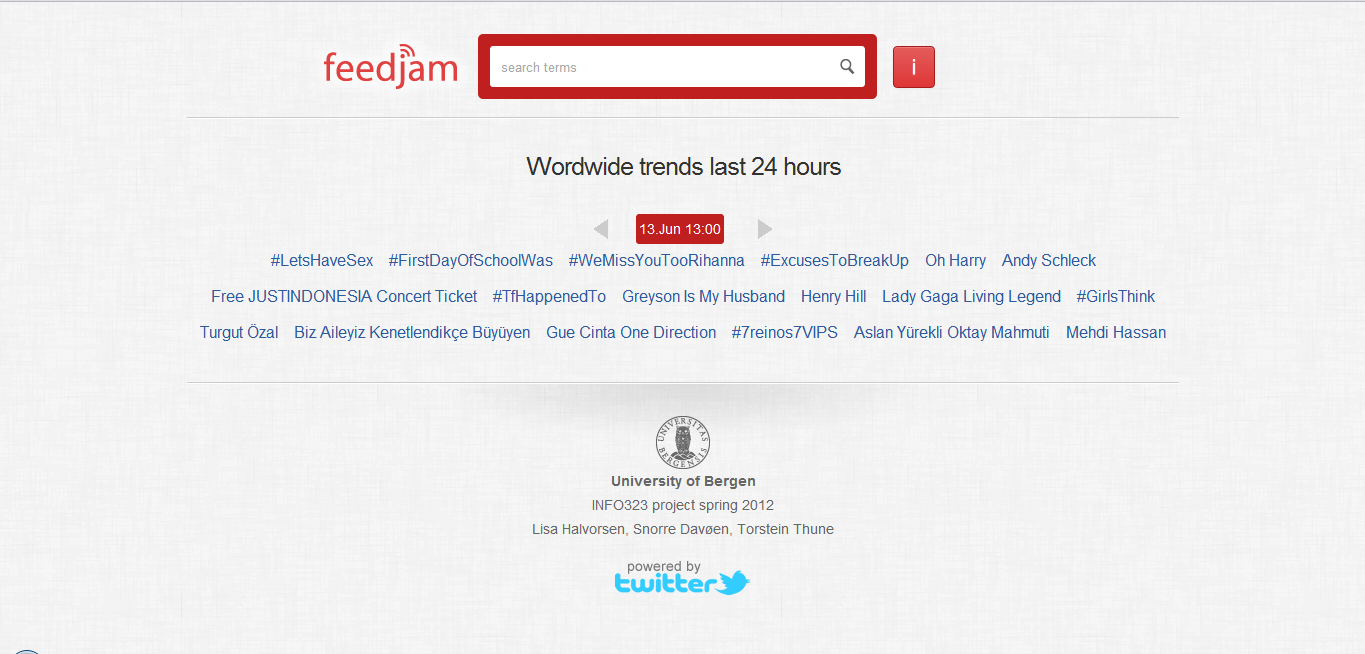
\includegraphics[width=1\textwidth]{figures/feedjam_frontpage_screenshot}
        \caption{The FeedJam frontpage}
        \label{fig:feedjamfrontpage}
    \end{minipage}
\end{figure}

\begin{figure}[ht]
    \begin{minipage}[b]{1\linewidth}
        \centering
        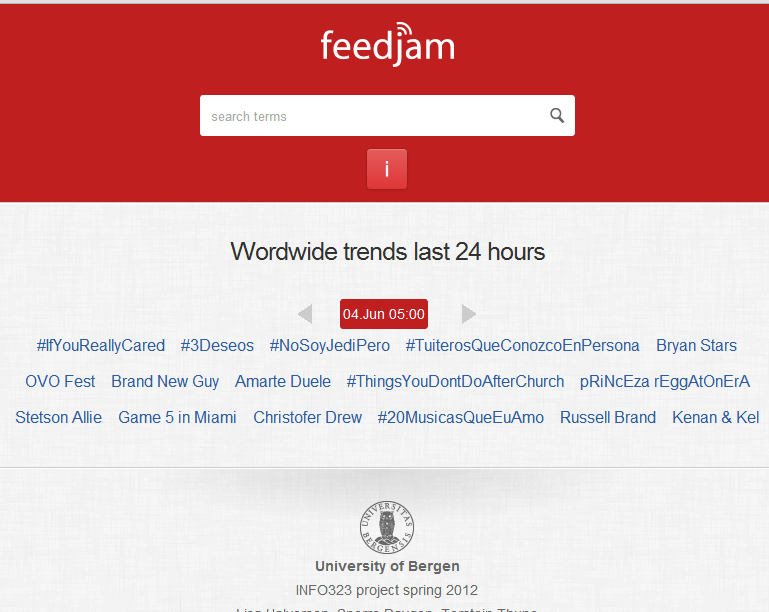
\includegraphics[width=1\textwidth]{figures/feedjam_responsive_frontpage}
        \caption{The FeedJam frontpage on lower resolutions}
        \label{fig:feedjamfrontpageresponsive}
    \end{minipage}
\end{figure}

\begin{figure}[ht]
    \begin{minipage}[b]{1\linewidth}
        \centering
        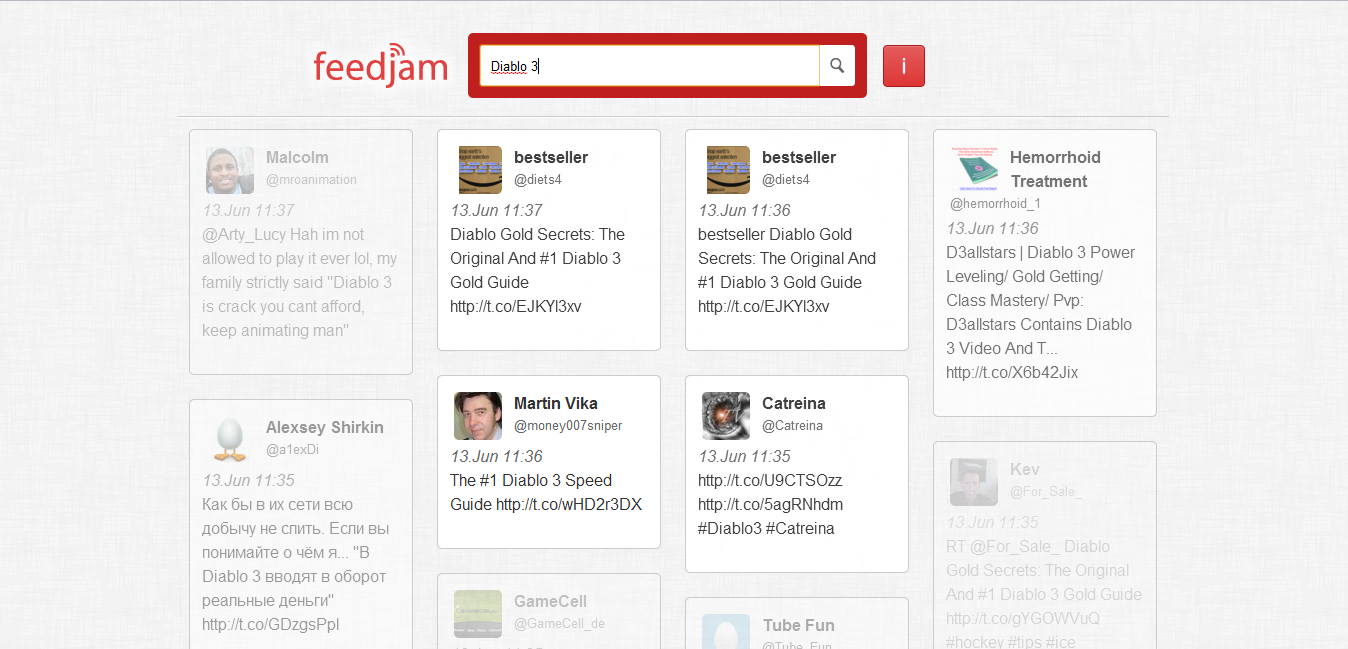
\includegraphics[width=1\textwidth]{figures/feedjam_search_screenshot}
        \caption{Search results}
        \label{fig:feedjamsearchresults}
    \end{minipage}
\end{figure}

\begin{figure}[ht]
    \begin{minipage}[b]{1\linewidth}
        \centering
        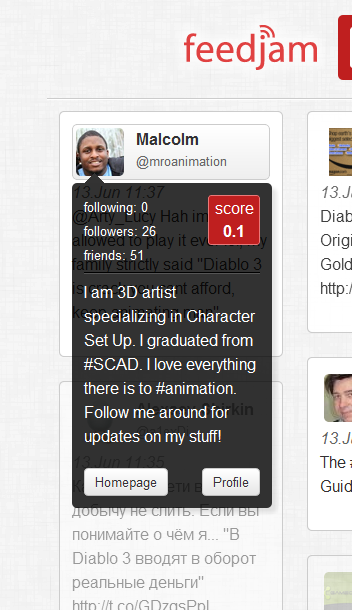
\includegraphics[width=0.7\textwidth]{figures/feedjam_user_screenshot}
        \caption{Displaying user information}
        \label{fig:feedjamuseropened}
    \end{minipage}
\end{figure}

\begin{figure}[ht]
    \begin{minipage}[b]{1\linewidth}
        \centering
        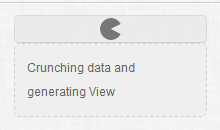
\includegraphics[width=1\textwidth]{figures/feedjam_loading}
        \caption{The FeedJam loading bar}
        \label{fig:feedjamloading}
    \end{minipage}
\end{figure}

\begin{figure}[ht]
    \begin{minipage}[b]{1\linewidth}
        \centering
        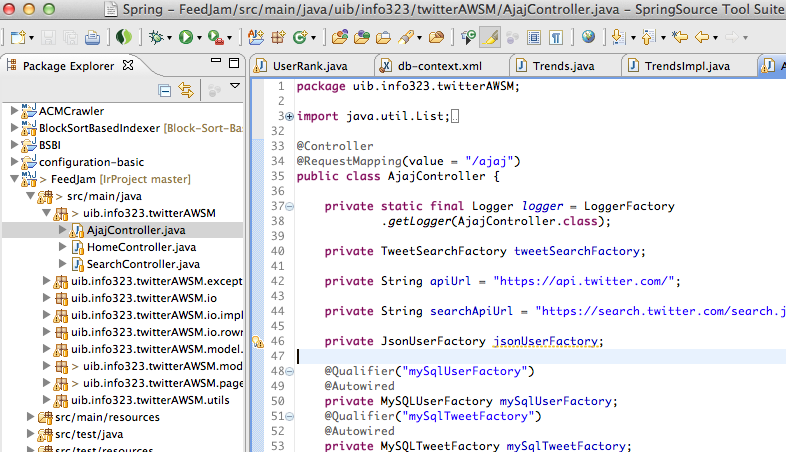
\includegraphics[width=1\textwidth]{figures/springsourcetoolsuite}
        \caption{The SpringSource Tool Suite IDE}
        \label{fig:springsourcetoolsuite}
    \end{minipage}
\end{figure}

\begin{figure}[ht]
    \begin{minipage}[b]{1\linewidth}
        \centering
        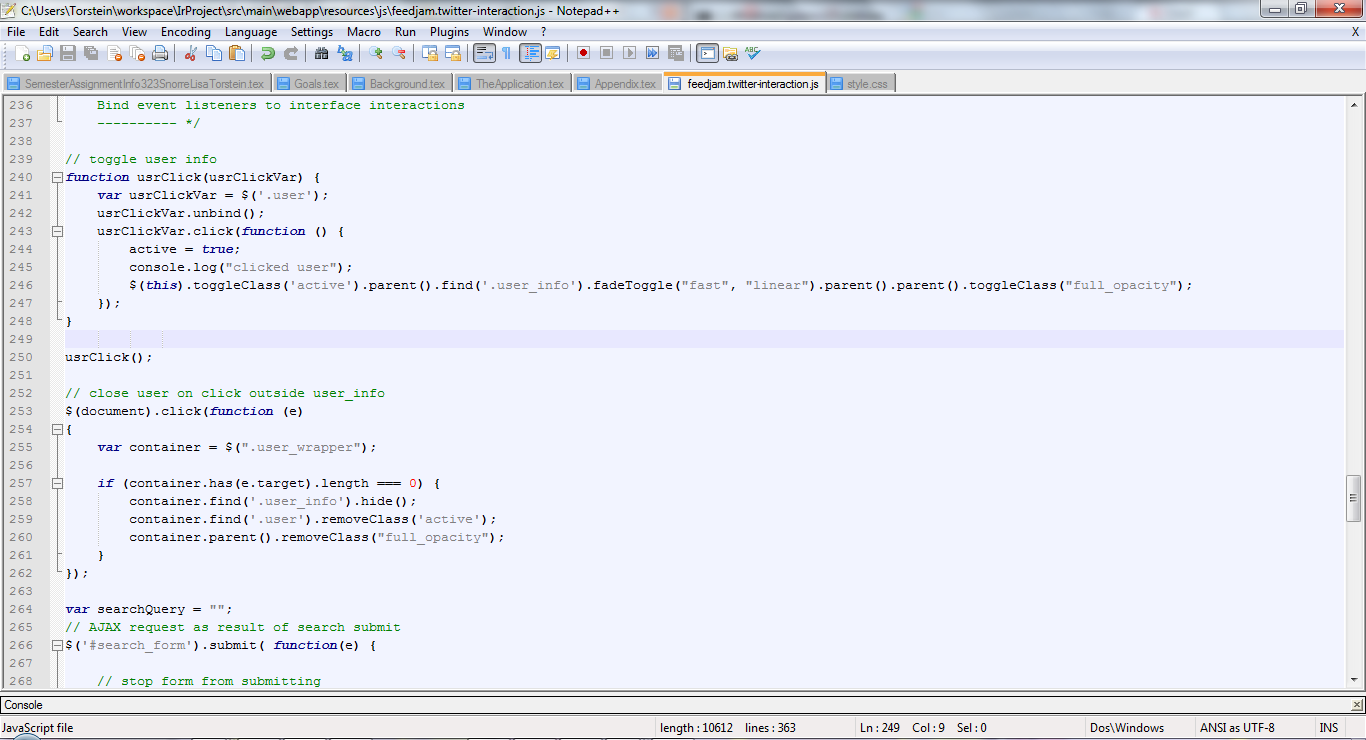
\includegraphics[width=1\textwidth]{figures/notepadplusplus}
        \caption{The Notepad++ text editor}
        \label{fig:notepadplusplus}
    \end{minipage}
\end{figure}

\begin{figure}[ht]
    \begin{minipage}[b]{1\linewidth}
        \centering
        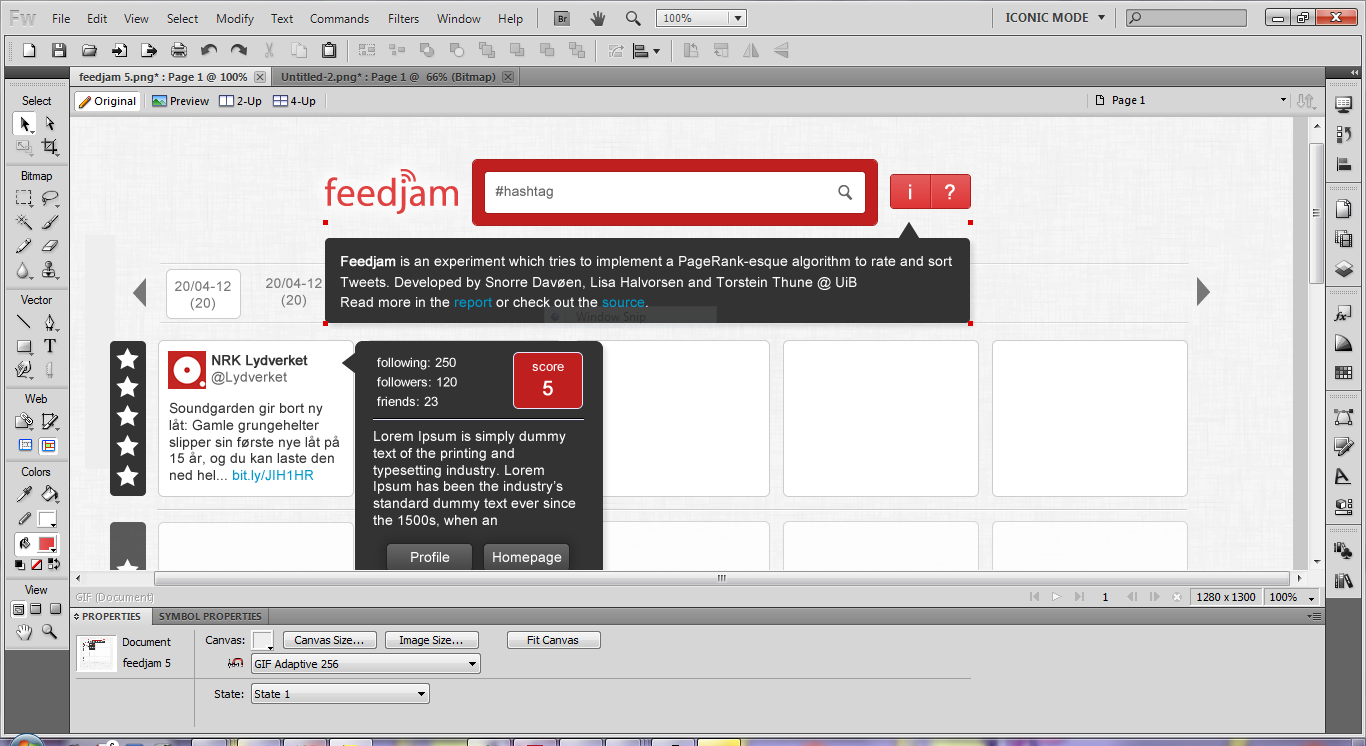
\includegraphics[width=1\textwidth]{figures/fireworks}
        \caption{Adobe Fireworks, a design/mockup utility}
        \label{fig:fireworks}
    \end{minipage}
\end{figure}

\begin{figure}[ht]
    \begin{minipage}[b]{1\linewidth}
        \centering
        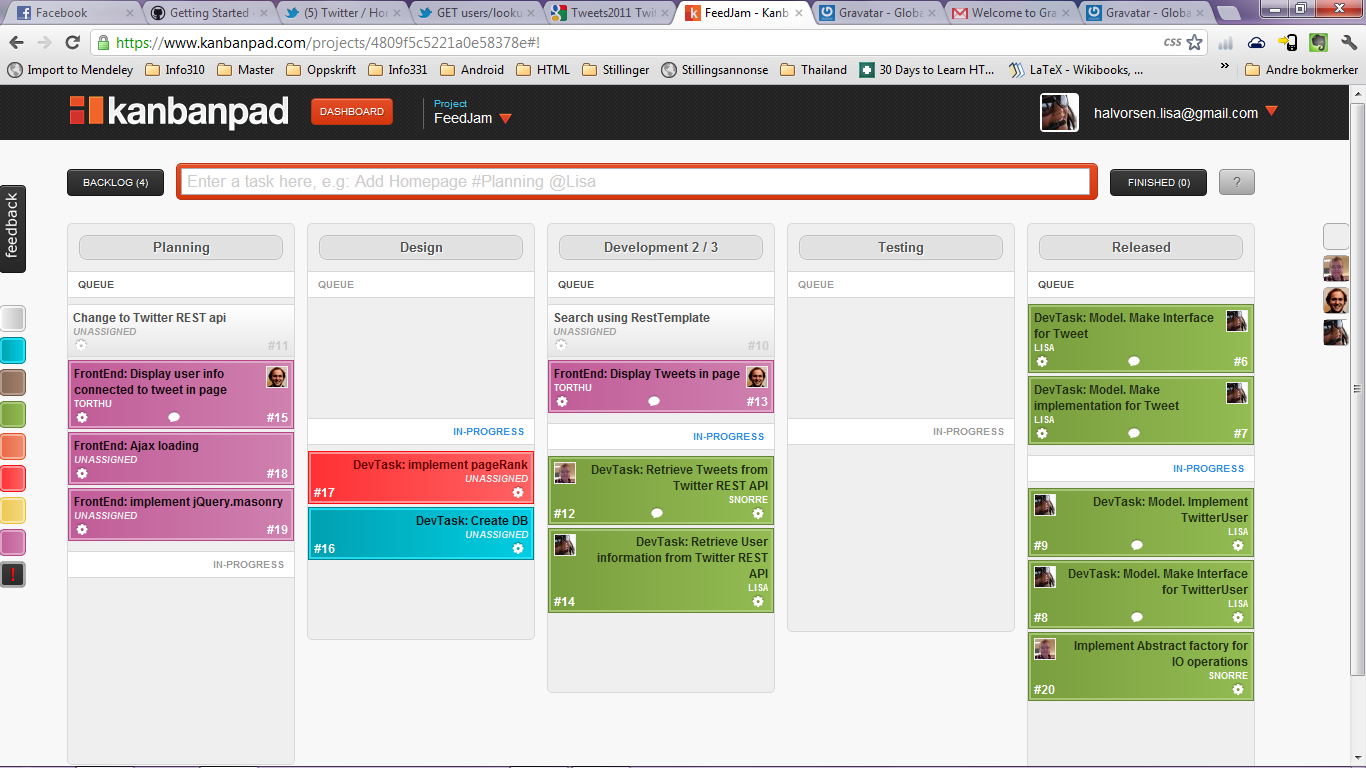
\includegraphics[width=1\textwidth]{figures/08052012}
        \caption{Screen shot of kanban board }
        \label{fig:kanbanScreenShot2}
    \end{minipage}
\end{figure}

\begin{figure}[ht]
    \begin{minipage}[b]{1\linewidth}
        \centering
        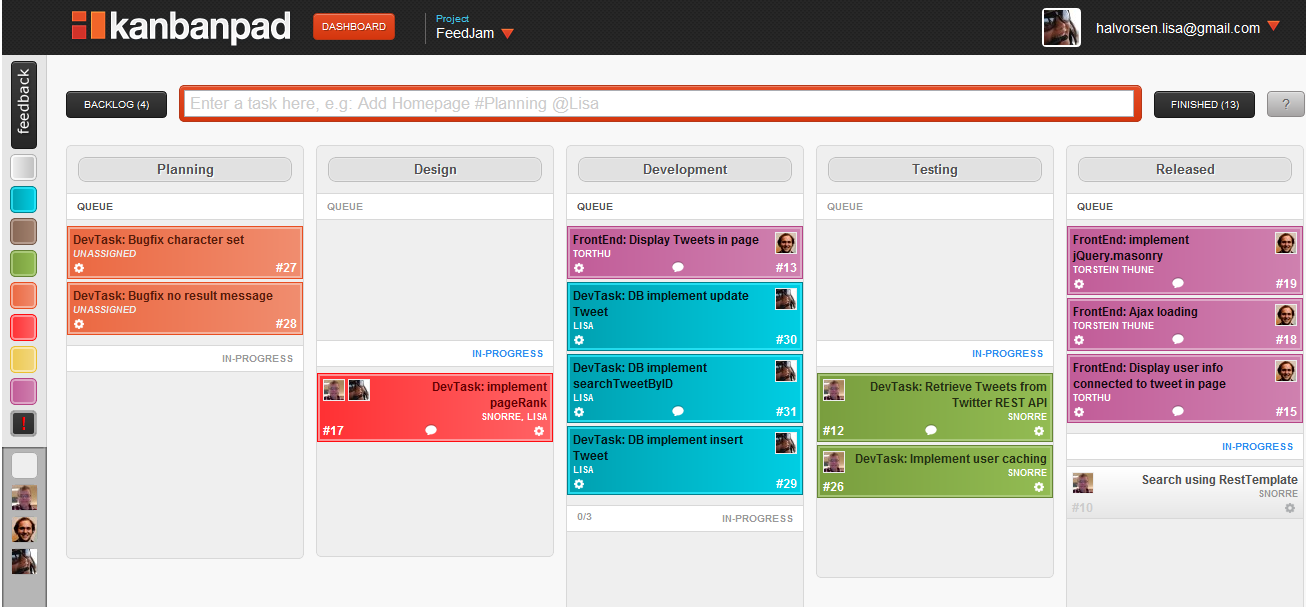
\includegraphics[width=1\textwidth]{figures/130512}
        \caption{Screen shot of kanban board }
        \label{fig:kanbanScreenShot}
    \end{minipage}
\end{figure}



\begin{figure}[ht]
    \begin{minipage}[b]{1\linewidth}
        \centering
        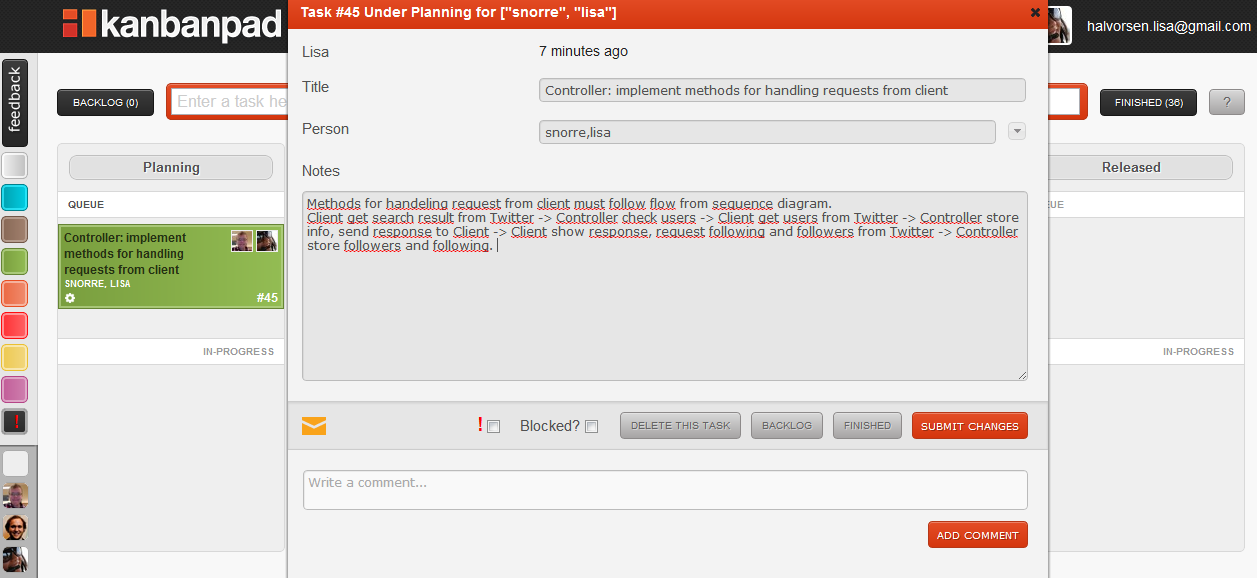
\includegraphics[width=1\textwidth]{figures/ajajcontroller}
        \caption{Screen shot of development task}
        \label{fig:kanbanScreenShotDevTask}
    \end{minipage}
\end{figure}

\end{document}
